\documentclass{beamer}
\usetheme{Madrid}

\usepackage{amsmath, amssymb, amsthm}
\usepackage{graphicx}
\usepackage{listings}
\usepackage{gensymb}
\usepackage[utf8]{inputenc}
\usepackage{hyperref}
\usepackage{gvv}

\begin{document}

\title{Assignment 11.9.5\_1Q}
\author{EE22BTECH11219 - Rada Sai Sujan$^{}$% <-this % stops a space
}
\frame{\titlepage}

\begin{frame}
\frametitle{Question}
Show that the sum of $\brak {m+n}^{th}$ and $\brak {m-n}^{th}$ terms of an $A.P.,$ is equal to twice the $m^{th}$ terms.    \\
\end{frame}

\begin{frame}{allowframebreaks}
\frametitle{Solution: Theory}
\begin{table}[ht]
    \centering
    \def\arraystretch{1.5}
    \begin{tabular}{|p{2cm}|p{6cm}|}
    \hline
    PARAMETER & DESCRIPTION \\ \hline
    $G_c$ & Proportional controller's transfer function \\ \hline
    $G_f$ & Valve transfer function \\ \hline
    $G_p$ & Process transfer function   \\ \hline
    $G_M$ & Measurement transfer function \\ \hline 
    $G\brak{s}$ & Open loop transfer function \\ \hline
    $T\brak{s}$ & Transfer function of system \\ \hline
\end{tabular}

    \caption{Parameter Table1}
    \label{tab:11.9.5.1.1}
\end{table}
\end{frame}

\begin{frame}
\frametitle{Theory}
For an $AP$,
\begin{align}
    x\brak{n}&=[x\brak{0}+nd]u\brak{n}   \\
    \implies x\brak{m+n}+x\brak{m-n}&=[x\brak{0}+\brak{m+n}d]+[x\brak{0}+\brak{m-n}d] \\
    &=2[x\brak{0}+md]   \\
    \therefore x\brak{m+n}+x\brak{m-n}&=2x\brak{m}
\end{align}
\end{frame}

\begin{frame}
\frametitle{Theory}
\begin{table}[ht]
    \centering
    \def\arraystretch{1.5}
    \begin{table}[htbp]
    \centering
    \def\arraystretch{1.5}
    \begin{tabular}{|p{4cm}|p{4cm}|}
    \hline
STATIONARY WAVE CONDITION & TRAVELLING WAVE CONDITION \\ \hline
        \brak 1 $A(x)$ should be a function of position x, and it can be expressed as $A(x)=A_{0}cos(\omega t+\alpha)$ where $A_{0}$ is a constant, $k$ is the wavenumber, $x$ is the position and $\alpha$ is a phase constant. & 
        \brak 1 $A(x)$ should be a constant, and it can be expressed as $A(x)=A_{0}$ where $A_{0}$ is a constant number. \\ \hline

        \brak 2 $\phi (x)$ can be expressed as $\phi (x)=c$ where c is a constant. &
        \brak 2 $\phi (x)$ is a linear expression in x or $\phi (x)=kx+\theta$ where k is the wavenumber and $\theta$ is the phaseconstant. \\ \hline
\end{tabular}
    \caption{Travelling wave $vs$ Stationary wave}
    \label{tab:table1}
\end{table}

    \caption{Verified Values}
    \label{tab:11.9.5.1.2}
\end{table}
\end{frame}

\begin{frame}
\frametitle{Code}
\begin{figure}[ht]
                        \centering
                        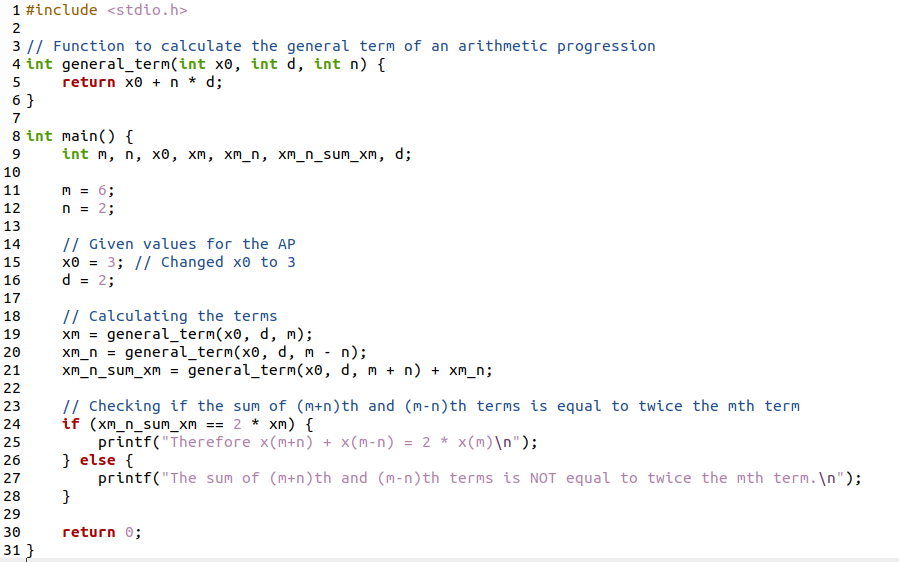
\includegraphics[width=\columnwidth]{figs/a.png}
                        \caption{DIPLACEMENT $vs$ TIME-graph1}
                        \label{fig:1}
\end{figure}
\end{frame}
\end{document}
